%==============================================================================
% Athena-SDA — Artigo de fundamentação e prova experimental
% Compilar a partir de docs/paper/:
%   pdflatex athena_sda_article.tex
%   pdflatex athena_sda_article.tex
% Figuras: figures/prepeak_*.png
%==============================================================================
\documentclass[11pt,a4paper]{article}

\usepackage[T1]{fontenc}
\usepackage[utf8]{inputenc}
\usepackage[brazil]{babel}
\usepackage{lmodern}
\usepackage{geometry}
\geometry{margin=2.2cm}
\usepackage{amsmath,amssymb,amsfonts}
\usepackage{booktabs}
\usepackage{graphicx}
\usepackage{hyperref}
\usepackage{xcolor}
\usepackage{setspace}
\usepackage{caption}
\usepackage{subcaption}
\usepackage{float}
\usepackage{url}
\usepackage{microtype}
\usepackage{enumitem}

\hypersetup{
  colorlinks=true,
  linkcolor=blue!50!black,
  citecolor=blue!50!black,
  urlcolor=blue!60!black
}

\title{\textbf{Athena-SDA:} detecção quantitativa de ruído orbital\\
e microanomalias em satélites de interesse militar\\
com Isolation Forest past-only e validação walk-forward\\
frente a âncoras open-source}

\author{
  Projeto Athena-SDA\\
  \texttt{https://github.com/CostaJr007/Athena-SDA}\\
  \small IBM SkillsBuild AI Builders --- \textit{Advance Space Exploration with AI}\\
  \small Fundamentação matemática e prova experimental (Claims~A+B)
}

\date{Agosto 2026}

\begin{document}
\maketitle
\begin{abstract}
\noindent
Apresentamos o \textbf{Athena-SDA}, um sistema de \textit{Space Domain Awareness} (SDA) com foco militar-first para \textbf{análise e detecção de ruído orbital} e \textbf{microanomalias de trajetória} em plataformas de interesse (\textit{suspects}), gerando \textbf{alertas operacionais} a partir de TLEs públicos e clima espacial GFZ.
Construímos um vetor de \textbf{features quantitativas} (entropia de Shannon, expoente de Hurst multi-escala, CUSUM, proxy de Kolmogorov, testes de estacionariedade, clima espacial F10.7/Ap/Kp, entre outras) e treinamos um \textbf{Isolation Forest} em âncoras de normalidade (\textit{baseline} civil e \textit{assets} protegidos), com protocolo \textbf{past-only}.
Validamos por \textbf{walk-forward} em janelas alinhadas a \textbf{reports open-source} e controlos \textbf{placebo} EO civis.
No painel GEO (Luch/Olymp-K, Shiyan-12, Luch-2): \textbf{5/5} hard hits com limiar $0{,}50$ e média do máximo de score $\approx 0{,}65$, versus \textbf{0/7} hard hits e média $\approx 0{,}46$ nos placebos EO (gap $\approx 0{,}19$; Mann--Whitney unilateral $p\approx 0{,}001$).
Uma camada de prioridade (XGBoost, pares suspect$\times$asset, fuzzy) e o copiloto Bob explicam e ordenam atenção sem alterar o score quant.
Definições resumidas de cada ferramenta matemática estão no \textbf{Glossário} (Apêndice~\ref{app:gloss}).
\end{abstract}

\tableofcontents
\vspace{0.8em}
\hrule
\vspace{1em}

%------------------------------------------------------------------------------
\section{Introdução}
\label{sec:intro}

Operadores de SDA não conseguem monitorar igualmente dezenas de milhares de objetos em órbita.
O Athena-SDA concentra-se em \textbf{análise quantitativa de séries orbitais} e em \textbf{deteção de ruído / microanomalias} em objetos de interesse militar, com geração de \textbf{alertas} e priorização de atenção face a plataformas a proteger.

O sistema combina:
\begin{enumerate}[leftmargin=*]
  \item dados públicos (TLE multi-anuais + clima espacial);
  \item um framework matemático de ruído (Sec.~\ref{sec:math});
  \item Isolation Forest past-only sob doutrina militar-first (Sec.~\ref{sec:if});
  \item validação walk-forward face a âncoras de reports e placebos (Sec.~\ref{sec:wf}--\ref{sec:results});
  \item camadas de prioridade e explicação (Sec.~\ref{sec:priority}).
\end{enumerate}

\paragraph{Pergunta de investigação.}
Um pipeline quant + Isolation Forest past-only, treinado em normalidade \textit{baseline}+\textit{asset}, separa estatisticamente janelas de interesse militar alinhadas a reports open-source de controlos EO civis no mesmo protocolo?

\paragraph{Claims formais.}
\begin{description}[style=nextline,leftmargin=12pt]
  \item[Claim A.] Cases de interesse (âncoras open-source) apresentam scores anómalos elevados e/ou hard hits perto de $t_{\mathrm{peak}}$.
  \item[Claim B.] Placebos EO civis, no mesmo protocolo, apresentam scores mais baixos e hard-hit rate próximo de zero em $\mathrm{thr}=0{,}50$.
\end{description}

%------------------------------------------------------------------------------
\section{Enquadramento e doutrina militar-first}
\label{sec:doctrine}

A watchlist Athena define três papéis operacionais:

\begin{center}
\begin{tabular}{@{}llp{7.2cm}@{}}
\toprule
\textbf{Papel} & \textbf{Exemplos} & \textbf{Uso no ML} \\
\midrule
\textit{asset} & ISS, GPS, DMSP, SAR aliado & Âncora de normalidade no IF; prioridade de proteção \\
\textit{suspect} & Luch/Olymp-K, Yaogan, Shiyan, CSS & Deteção primária de microanomalia / ruído \\
\textit{baseline} & TERRA, AQUA, Landsat, NOAA & Treino do IF (referência de órbita estável) \\
\bottomrule
\end{tabular}
\end{center}

\textit{Suspects} não entram no treino de normalidade do Isolation Forest.
Constelações comerciais (ex.\ Starlink) são excluídas desse treino para não definir o padrão de normalidade militar.
O produto de análise é a watchlist e o pipeline quant; a UI 3D é de demonstração.

%------------------------------------------------------------------------------
\section{Dados}
\label{sec:data}

\subsection{Séries orbitais (TLE)}
\begin{itemize}[leftmargin=*]
  \item Histórico filtrado para 24 NORADs ($\sim$2014-01-01 a 2026-07-27), $\sim$\textbf{249\,580} épocas.
  \item Origem: espelho público de história TLE + ingestão diária CelesTrak GP.
  \item Elementos: semi-eixo maior (SMA), excentricidade, inclinação, RAAN, movimento médio, \textit{timestamps}.
\end{itemize}

\subsection{Clima espacial}
Fonte \textbf{GFZ Potsdam} (Kp, ap/Ap, F10.7 observado/ajustado, manchas):
\begin{itemize}[leftmargin=*]
  \item $F_{10.7}$, $F_{10.7}^{\mathrm{adj}}$, $\mathrm{Ap}$, $\overline{K_p}$, número de manchas;
  \item médias e deltas em 7 dias;
  \item \texttt{geomagnetic\_storm}$=1$ se $\mathrm{Ap}_{\max,7\mathrm{d}}\ge 30$.
\end{itemize}
O clima espacial entra no vetor de features para contextualizar arrasto atmosférico (especialmente LEO) face a mudanças de SMA.

\subsection{Âncoras open-source}
Eventos em \texttt{events\_walkforward.json} com $(t_{\mathrm{start}}, t_{\mathrm{peak}}, t_{\mathrm{end}})$ e fontes públicas (Gunter, CSIS, SWF, imprensa, catálogo dual-use). Exemplos: Luch/Olymp-K e Intelsat/Athena-Fidus; Shiyan-12; Luch-2; CSS Tianhe; placebos TERRA, AQUA, Landsat, NOAA.

%------------------------------------------------------------------------------
\section{Vetor de ruído quantitativo}
\label{sec:math}

Seja $a(t)$ a série de semi-eixo maior (km) na janela de $n\ge 20$ épocas.
O motor \texttt{src/engine.py} produz o vetor $x\in\mathbb{R}^{d}$ usado pelo Isolation Forest.
(Explicação resumida de cada ferramenta: Apêndice~\ref{app:gloss}.)

\subsection{Entropia de Shannon}
Diferenças $\Delta a_i = a_{i+1}-a_i$, histograma $p_k$:
\begin{equation}
  H = -\sum_{k:\,p_k>0} p_k \log_2 p_k .
\end{equation}

\subsection{Proxy de complexidade de Kolmogorov}
Tokens $\{U,D,S\}$ sobre $\Delta a$ e compressão zlib:
\begin{equation}
  K_{\mathrm{proxy}} = \mathrm{clip}\!\left(\frac{\ell_{\mathrm{comp}}}{\ell_{\mathrm{raw}}},\,0,\,1\right).
\end{equation}

\subsection{Expoente de Hurst (R/S) multi-escala}
$H$ na janela completa e no trecho curto recente; gap
\begin{equation}
  \Delta H = H_{\mathrm{full}} - H_{\mathrm{short}}.
\end{equation}

\subsection{CUSUM-$L_1$ kernelizado}
Desvios acumulados face a mediana local / MAD, mapeados em $[0,1]$.

\subsection{Cauda de Mandelbrot / Hill}
Score de extremos da série acima de quantil (cauda pesada).

\subsection{ADF}
$p$-valor do teste Dickey--Fuller aumentado sobre $a(t)$.

\subsection{Deltas e manobras}
$\Delta$SMA 7d/30d e contagem de picos tipo manobra via CUSUM.

\subsection{Topologia e geometria (proxies)}
Homologia H0/H1 (modo proxy por distâncias normalizadas), Chern--Simons proxy sobre $h=r\times v$, Ricci--Ollivier proxy por Wasserstein local.
Reconstrução a partir de elementos orbitais (não SGP4 completo).

\subsection{Clima espacial}
$F_{10.7}$, Ap, Kp e derivados de 7 dias no mesmo vetor $x$.

\subsection{Fora do IF}
Distância a assets e cointegração entram na camada de prioridade, não no Isolation Forest de ruído da série.

%------------------------------------------------------------------------------
\section{Isolation Forest past-only}
\label{sec:if}

Score unificado:
\begin{equation}
  s(x) = \mathrm{clip}\bigl(0{,}5 - \mathrm{decision\_function}(x),\, 0,\, 1\bigr).
\end{equation}

\paragraph{Treino.}
Janelas com $\mathrm{window\_end}<\mathrm{cutoff}$; NORADs \textbf{baseline + asset}; contamination $\sim 0{,}06$--$0{,}08$; \texttt{random\_state=42}; modelos monitor e pipeline separados (\texttt{registry.json}).

\paragraph{Limiar.}
\begin{equation}
  thr = \max\bigl(0{,}50,\, p_{95}(s_{\mathrm{normality}})\bigr).
\end{equation}
Tabelas principais: $\mathrm{thr}=0{,}50$.

\paragraph{Hard hit.}
Fold com $s\ge 0{,}50$ em $[t_{\mathrm{peak}}\pm 45\,\mathrm{d}]$.

%------------------------------------------------------------------------------
\section{Protocolo walk-forward}
\label{sec:wf}

Para cada evento $(t_{\mathrm{start}}, t_{\mathrm{peak}}, t_{\mathrm{end}})$:
\begin{enumerate}[leftmargin=*]
  \item Grelha \texttt{asof} com passo 14 dias.
  \item Em cada \texttt{asof}: IF treinado só com janelas de normalidade terminando antes de \texttt{asof}$-3$ dias.
  \item Score do NORAD alvo na janela corrente.
  \item Métricas: hard hit, $\max s$, média pre-peak, \texttt{noise\_ramp}, \texttt{first\_fold\_hit}.
\end{enumerate}
Protocolo fixado em \texttt{PROTOCOL\_PREREGISTRATION.md}.

%------------------------------------------------------------------------------
\section{Camada de prioridade}
\label{sec:priority}

Complementa a detecção de ruído para ordenar atenção do operador:
\begin{itemize}[leftmargin=*]
  \item XGBoost com weak labels (níveis operacionais);
  \item distância e cointegração suspect$\times$asset (\texttt{pair\_risk});
  \item fuzzy Mamdani e critério de Kelly (atenção);
  \item Bob: texto explicativo a partir dos scores já calculados.
\end{itemize}
Claims A+B usam apenas o score IF do walk-forward.

%------------------------------------------------------------------------------
\section{Desenho experimental}
\label{sec:design}

\paragraph{Painel GEO (principal).}
Interest: 5 eventos (Luch-1 $\times$3, SY-12, Luch-2), 3 NORADs únicos.
Placebos EO: 7 janelas (TERRA, AQUA, Landsat, NOAA), 5 NORADs únicos.

\paragraph{Painel expandido.}
Até 9 NORADs únicos de interesse (LEO/MEO incluídos); reportado em separado.

\paragraph{Separação.}
Mann--Whitney $U$ unilateral (interest $>$ placebo), com ênfase em médias e gap.

%------------------------------------------------------------------------------
\section{Resultados}
\label{sec:results}

\subsection{Claims A+B --- painel GEO}
\begin{table}[H]
\centering
\caption{Resultados principais (thr$=0{,}50$, past-only). Fonte: \texttt{paper\_validation\_latest.json}.}
\label{tab:geo}
\begin{tabular}{@{}lcccc@{}}
\toprule
Grupo & $n$ eventos & Hard hit & Média $\max s$ & Média pre-peak \\
\midrule
Interest GEO & 5 & \textbf{5/5 (100\%)} & \textbf{0{,}651} & \textbf{0{,}567} \\
Placebo EO civil & 7 & \textbf{0/7 (0\%)} & 0{,}462 & 0{,}385 \\
\midrule
Gap (interest $-$ placebo) & & & \textbf{0{,}189} & --- \\
Mann--Whitney (max) & & & $p\approx 0{,}0013$ & --- \\
\bottomrule
\end{tabular}
\end{table}

O pipeline quant+IF separa regimes de ruído elevados nos cases GEO de interesse face aos placebos EO (\textbf{Claims A e B suportados} neste painel).

\subsection{Amostra por evento}
\begin{table}[H]
\centering
\caption{Scores por evento (amostra).}
\label{tab:events}
\scriptsize
\begin{tabular}{@{}llccc@{}}
\toprule
Evento & NORAD & Hard & $\max s$ & Pre-peak mean \\
\midrule
luch1\_intelsat\_2015 & 40258 & sim & 0{,}628 & 0{,}570 \\
luch1\_intelsat\_mid2015 & 40258 & sim & 0{,}675 & 0{,}589 \\
luch1\_athena\_fidus\_2018 & 40258 & sim & 0{,}672 & 0{,}560 \\
sy12\_geo\_rpo\_2021\_22 & 50321 & sim & 0{,}623 & 0{,}529 \\
luch2\_trailing\_2023 & 55841 & sim & 0{,}658 & 0{,}586 \\
tianhe\_css\_assembly\_2021 & 48274 & sim & 0{,}644 & 0{,}556 \\
placebo\_terra\_2015 & 25994 & não & 0{,}481 & 0{,}395 \\
placebo\_aqua\_2015 & 27424 & não & 0{,}474 & 0{,}429 \\
placebo\_landsat8\_2018 & 39084 & não & 0{,}460 & 0{,}367 \\
placebo\_noaa20\_2023 & 43013 & não & 0{,}464 & 0{,}391 \\
\bottomrule
\end{tabular}
\end{table}

\subsection{Curvas de score}
As Figuras~\ref{fig:luch}--\ref{fig:grids} mostram $s(\mathrm{asof})$, limiar $0{,}50$ e $t_{\mathrm{peak}}$.

\begin{figure}[H]
  \centering
  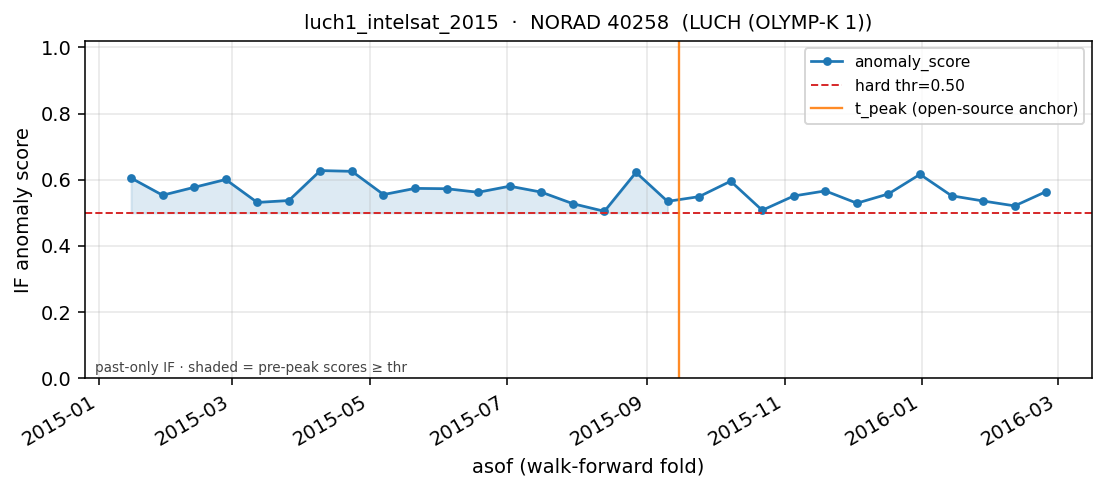
\includegraphics[width=0.92\textwidth]{figures/prepeak_luch1_intelsat_2015.png}
  \caption{Luch-1 / Olymp-K (40258), episódio Intelsat 2015.}
  \label{fig:luch}
\end{figure}

\begin{figure}[H]
  \centering
  \begin{subfigure}[t]{0.48\textwidth}
    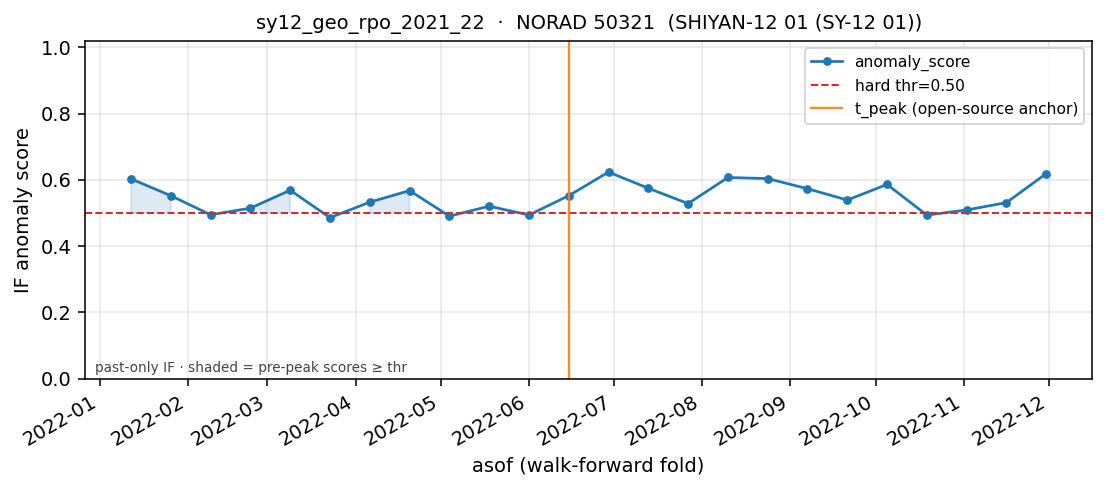
\includegraphics[width=\textwidth]{figures/prepeak_sy12_geo_rpo_2021_22.png}
    \caption{Shiyan-12 (50321).}
  \end{subfigure}\hfill
  \begin{subfigure}[t]{0.48\textwidth}
    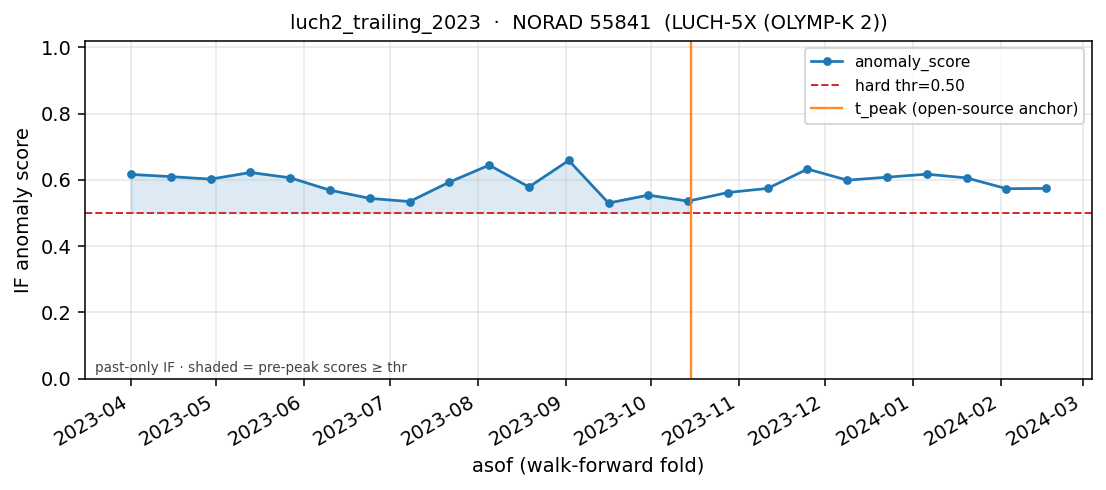
\includegraphics[width=\textwidth]{figures/prepeak_luch2_trailing_2023.png}
    \caption{Luch-2 (55841).}
  \end{subfigure}
  \caption{Cases de interesse com NORADs distintos.}
  \label{fig:sy12luch2}
\end{figure}

\begin{figure}[H]
  \centering
  \begin{subfigure}[t]{0.48\textwidth}
    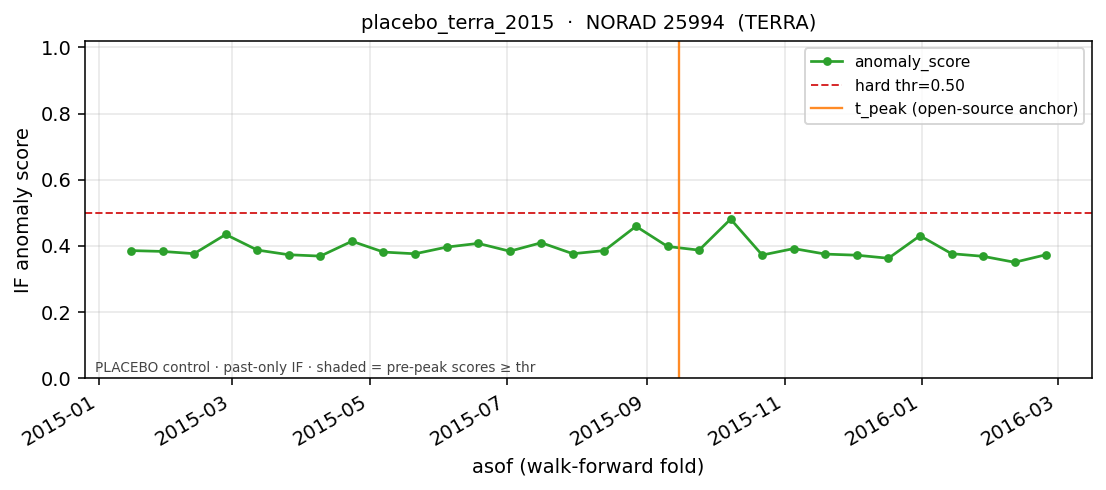
\includegraphics[width=\textwidth]{figures/prepeak_placebo_terra_2015.png}
    \caption{Placebo TERRA 2015.}
  \end{subfigure}\hfill
  \begin{subfigure}[t]{0.48\textwidth}
    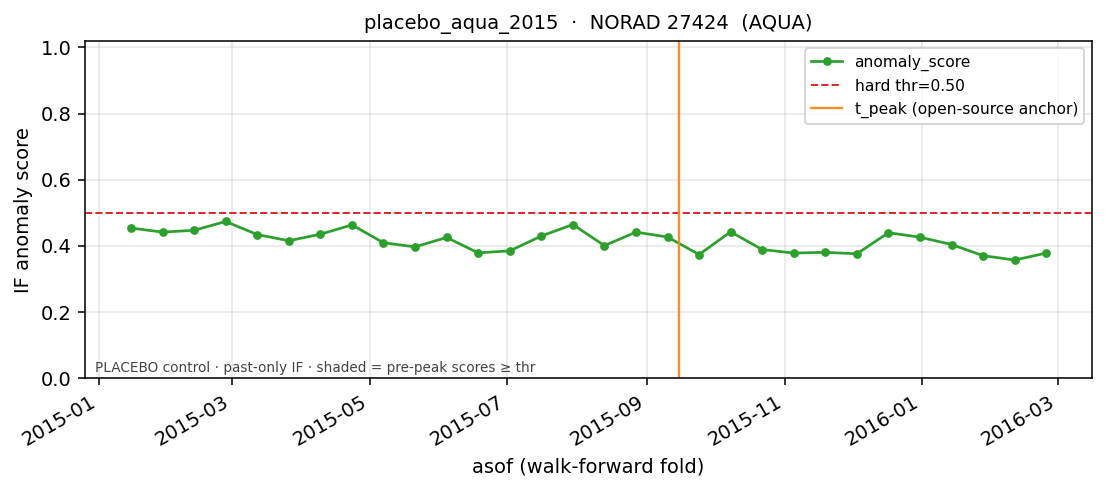
\includegraphics[width=\textwidth]{figures/prepeak_placebo_aqua_2015.png}
    \caption{Placebo AQUA 2015.}
  \end{subfigure}
  \caption{Controlos EO civis.}
  \label{fig:placebo}
\end{figure}

\begin{figure}[H]
  \centering
  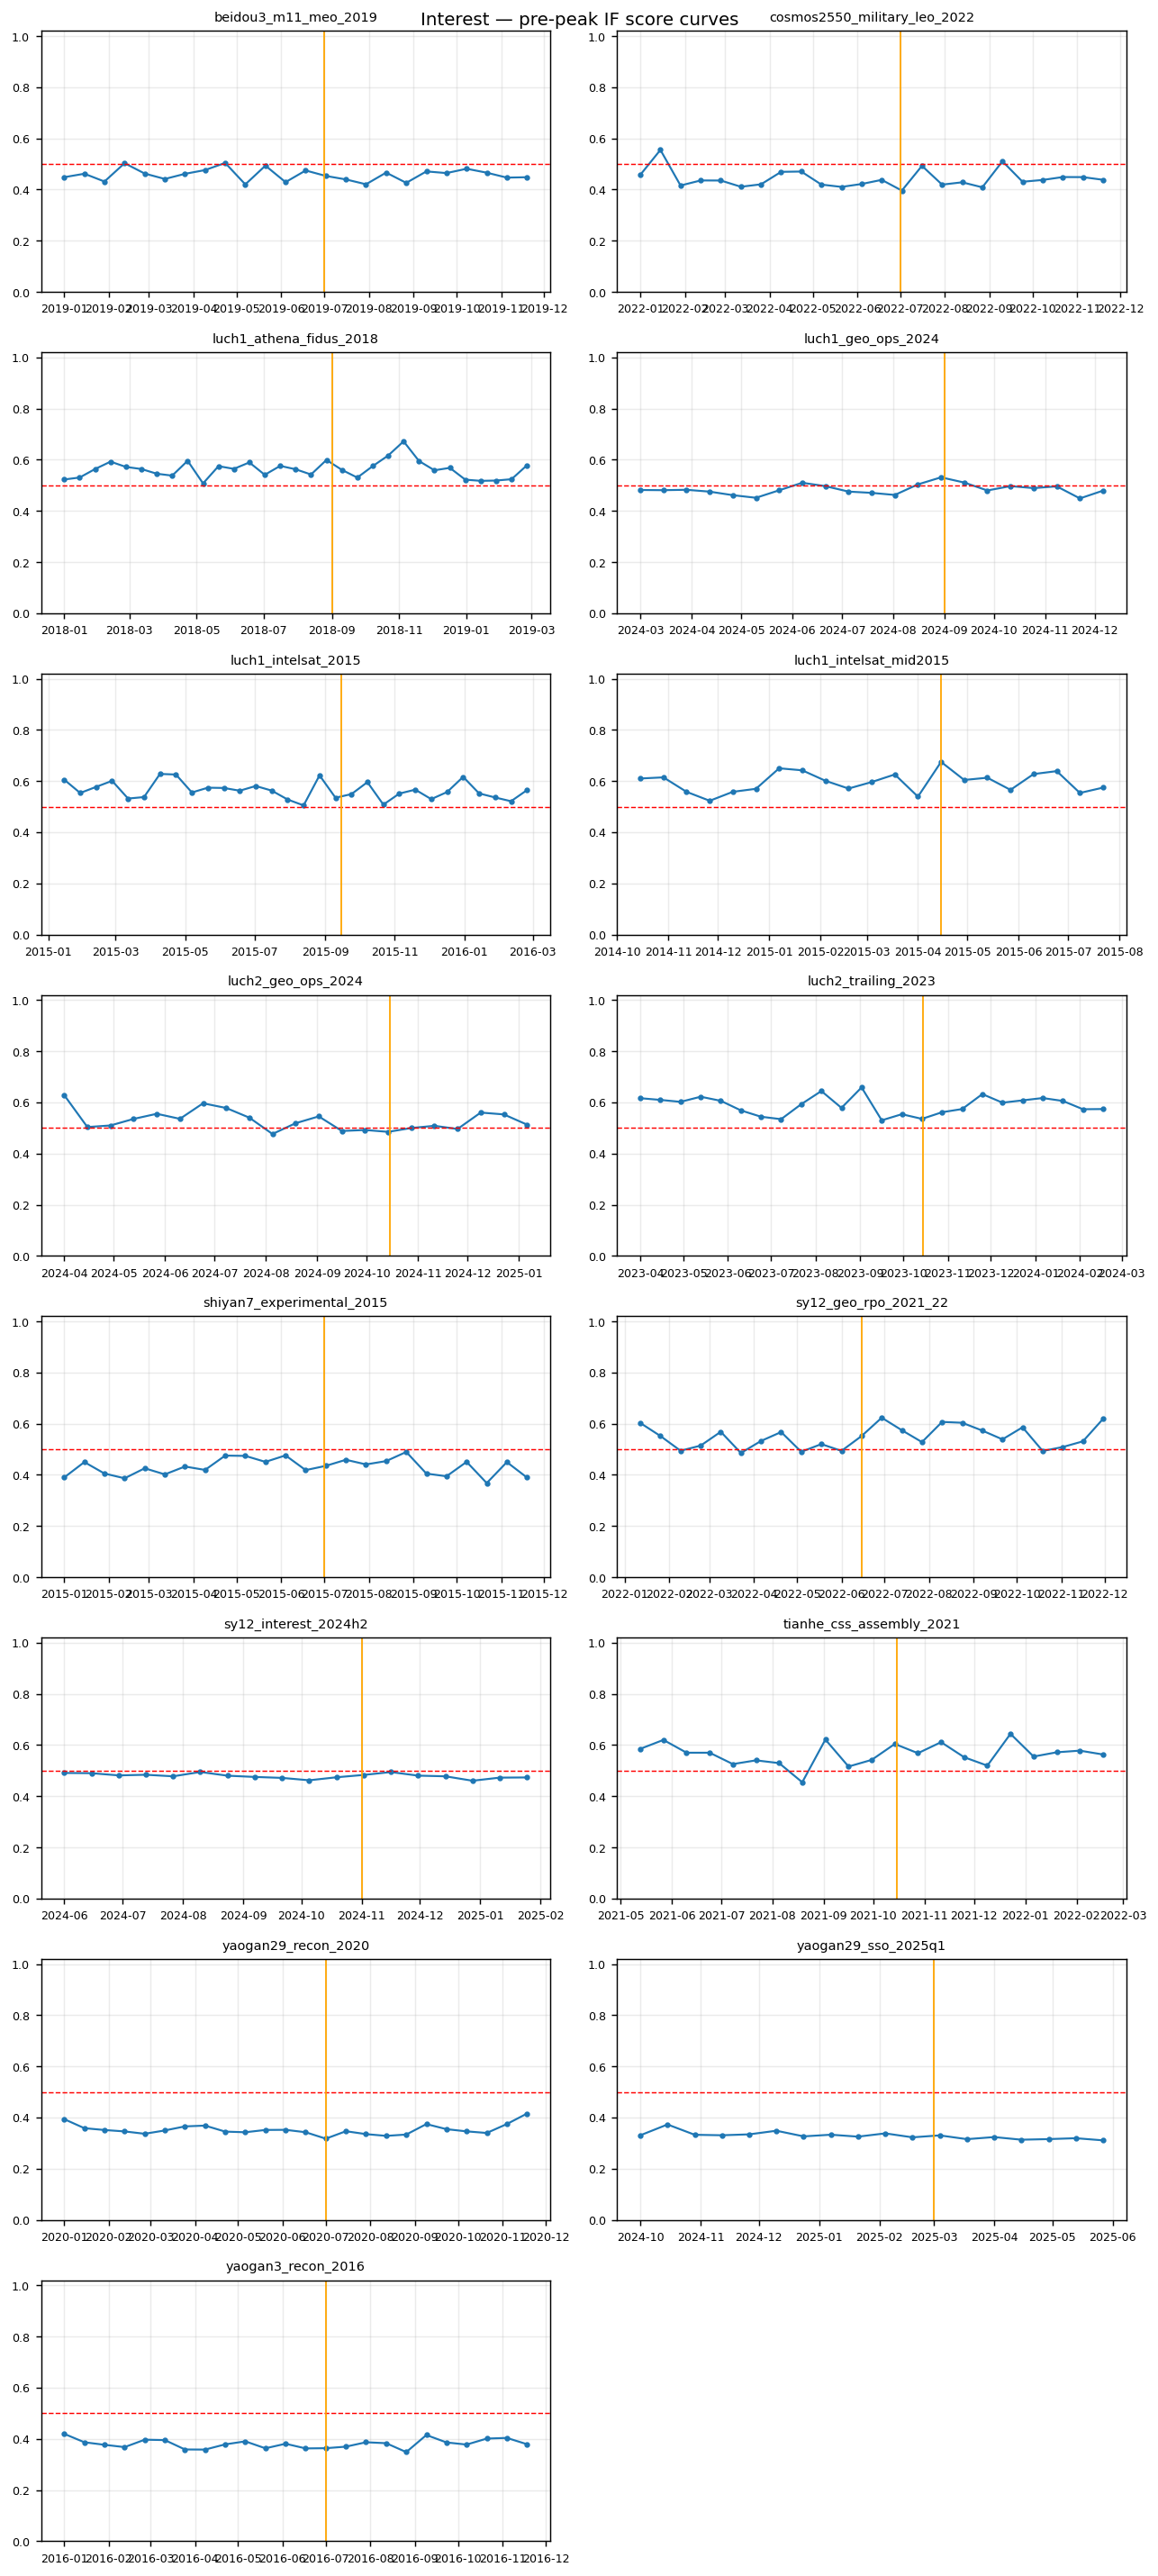
\includegraphics[width=0.95\textwidth]{figures/prepeak_grid_interest.png}
  \caption{Grelha de curvas de interesse.}
  \label{fig:grids}
\end{figure}

\subsection{Painel expandido}
Com 11 eventos / 9 NORADs únicos de interesse, hard-hit rate $\approx 55\%$ (LEO nem sempre $\ge 0{,}50$), com gap de médias ainda positivo face aos placebos (MW $p\approx 0{,}01$). O resultado principal do artigo é o painel GEO.

%------------------------------------------------------------------------------
\section{Discussão}
\label{sec:discussion}

Os resultados mostram que o score $s(x)$ responde a regimes de ruído elevados nos cases GEO de interesse alinhados a âncoras open-source, com separação clara face a EO civil.
Muitos cases apresentam nível pre-peak alto e \texttt{noise\_ramp} próximo de zero, coerente com \textbf{regime elevado persistente} na janela de análise.
O clima espacial contextualiza arrasto; a prioridade (pares, XGB) ordena atenção quando há proximidade a assets.

%------------------------------------------------------------------------------
\section{Limitações}
\label{sec:limits}

\begin{itemize}[leftmargin=*]
  \item $N$ pequeno de NORADs únicos; Luch-1 multi-evento é dependente.
  \item TLE esparso e ruidoso; proxies topológicos sobre reconstrução.
  \item LEO recon/dual-use com hard-hit menos frequente no thr $0{,}50$.
  \item Accuracy XGB mede weak labels, não a prova A+B.
\end{itemize}

%------------------------------------------------------------------------------
\section{Reprodutibilidade}
\label{sec:repro}

\begin{verbatim}
python scripts/run_anomaly_monitor.py train-baseline --holdout-days 1
python scripts/run_paper_validation.py --run-wf --threshold 0.50
python scripts/plot_prepeak_curves.py
cd docs/paper && pdflatex athena_sda_article.tex
\end{verbatim}

%------------------------------------------------------------------------------
\section{Conclusão}
\label{sec:concl}

O Athena-SDA implementa análise e detecção quantitativa de ruído orbital e microanomalias em watchlist militar-first, com Isolation Forest past-only e validação walk-forward.
No painel GEO, Claims A e B são suportados (5/5 vs 0/7 hard hits; gap $\approx 0{,}19$).
O glossário no apêndice resume o papel de cada ferramenta matemática usada no vetor de features.

%==============================================================================
\appendix
\section{Glossário das ferramentas matemáticas e de modelo}
\label{app:gloss}

Cada entrada resume \textbf{o que a ferramenta faz} no Athena-SDA (sem reabrir o corpo do artigo).

\begin{description}[style=nextline,leftmargin=8pt,font=\normalfont\bfseries]
  \item[Entropia de Shannon]
  Mede o quão ``espalhada'' ou irregular é a distribuição dos passos de altitude ($\Delta$SMA). Valores altos: sequência de mudanças menos previsível (controlo irregular / ops ativas).

  \item[Proxy de Kolmogorov]
  Estima se o padrão sobe/desce/estável da série é difícil de comprimir. Valores altos: padrão de manobra mais elaborado ou irregular face a um padrão simples.

  \item[Expoente de Hurst (R/S)]
  Mede persistência temporal: se desvios tendem a continuar na mesma direção. $H>0{,}5$: tendência/controlo persistente (útil para microtrajetória / low-thrust aparente).

  \item[Hurst multi-escala / $\Delta H$]
  Compara persistência da janela completa com a ponta recente. Destaca memória longa versus flutuação só no trecho final.

  \item[CUSUM-$L_1$]
  Detecta quebra de regime: acumula desvios face ao nível recente (mediana/MAD). Elevado quando a série ``muda de patamar''.

  \item[Mandelbrot / Hill (cauda)]
  Realça saltos raros e extremos na série de altitude (impulsos ou eventos pontuais fortes).

  \item[ADF (Dickey--Fuller)]
  Testa se a série é estacionária ou anda à deriva. $p$ alto favorece regime não mean-reverting.

  \item[$\Delta$SMA e contagem de manobras]
  Quantificam magnitude e frequência de mudanças de semi-eixo (relocação, ops intensas).

  \item[Homologia H0/H1 (proxy)]
  Resume estrutura da nuvem de posições reconstruídas (conectividade / ciclos em escala). Apoio geométrico global.

  \item[Chern--Simons (proxy)]
  Mede variação do momento angular específico na reconstrução $r,v$ --- indício de desvio de dinâmica Kepleriana ideal.

  \item[Ricci--Ollivier (proxy)]
  Mede distorção local entre vizinhanças na nuvem de pontos (curvatura discreta).

  \item[Clima espacial (F10.7, Ap, Kp, storm)]
  Contextualiza atividade solar e geomagnética. Ajuda a interpretar $\Delta$SMA em LEO sob arrasto elevado.

  \item[Isolation Forest]
  Modelo não supervisionado que isola perfis raros no espaço de features. Score alto = combinação de sinais pouco típica face às âncoras de normalidade.

  \item[Walk-forward past-only]
  Em cada data histórica, o IF só vê o passado. Avalia se o score sobe em janelas de eventos reais e placebos.

  \item[Cointegração]
  Testa se duas séries de altitude partilham tendência comum (padrão de movimento conjunto / escolta).

  \item[Distância suspect$\times$asset]
  Proximidade orbital aproximada para priorizar atenção a assets protegidos.

  \item[XGBoost (weak labels)]
  Classificador de prioridade operacional a partir de regras heurísticas de treino. Não define o hard hit da prova A+B.

  \item[Fuzzy Mamdani]
  Regras linguísticas com graus de pertinência para calibrar saída sob incerteza (ex.\ TLE antigo).

  \item[Kelly]
  Heurística de dimensionamento de atenção/recurso a partir de score e severidade.

  \item[Bob]
  Camada de texto que descreve scores e contexto; não recalcula o IF.
\end{description}

\begin{thebibliography}{99}
\bibitem{shannon1948}
C.~E. Shannon, ``A mathematical theory of communication,'' \textit{Bell Syst. Tech. J.}, 1948.

\bibitem{hurst1951}
H.~E. Hurst, ``Long-term storage capacity of reservoirs,'' \textit{Trans. Amer. Soc. Civ. Eng.}, 1951.

\bibitem{kolmogorov1965}
A.~N. Kolmogorov, ``Three approaches to the quantitative definition of information,'' 1965.

\bibitem{iforest2008}
F.~T. Liu, K.~M. Ting, and Z.-H. Zhou, ``Isolation Forest,'' in \textit{ICDM}, 2008.

\bibitem{engle1987}
R.~F. Engle and C.~W.~J. Granger, ``Co-integration and error correction,'' \textit{Econometrica}, 1987.

\bibitem{mandelbrot1963}
B.~Mandelbrot, ``The variation of certain speculative prices,'' \textit{J. Business}, 1963.

\bibitem{gfz}
J.~Matzka et al., Geomagnetic Kp index, GFZ Potsdam.

\bibitem{athena}
Athena-SDA: \url{https://github.com/CostaJr007/Athena-SDA}, \texttt{docs/paper/*}.
\end{thebibliography}

\end{document}
